\documentclass[10pt,border=3mm,tikz]{standalone}
\usetikzlibrary{arrows.meta}
\usetikzlibrary{decorations.pathmorphing}

\begin{document}
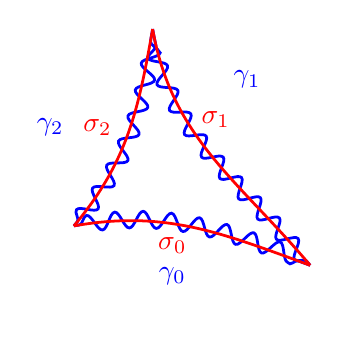
\begin{tikzpicture}[
    inner/.style={red,line width = 1pt,},
    inner_2/.style={blue,line width = 1pt,decorate,decoration={snake,amplitude=3pt,pre length=2pt,post length=3pt}},
    arr/.style={<->,cyan,dotted,line width=.6pt},
 ]
    % ~~~ the 3 points ~~~~~~~~~~~~~
    \coordinate (A) at (0,0);
    \coordinate (B) at (3,-.5);
    \coordinate (C) at (1,2.5);
    
    %Lines
    \draw[inner_2] (A) to[out= 10,in=160] coordinate [pos=.55] (A1) (B);
    \draw[inner_2] (A) to[out= 50,in=260] coordinate [pos=.30] (C1) (C);
    \draw[inner_2] (B) to[out=130,in=280] coordinate [pos=.40] (B1) (C);

    \draw[inner] (A) to[out= 10,in=160] coordinate [pos=.55] (A1) (B);
    \draw[inner] (A) to[out= 50,in=260] coordinate [pos=.30] (C1) (C);
    \draw[inner] (B) to[out=130,in=280] coordinate [pos=.40] (B1) (C);

    %Text

    \node[label={[text = blue]$\gamma_0$}] at (1.25,-1) {};
    \node[label={[text = blue]$\gamma_1$}] at (2.2,1.5) {};
    \node[label={[text = blue]$\gamma_2$}] at (-0.3,0.9) {};

    \node[label={[text = red]$\sigma_0$}] at (1.25,-0.6) {};
    \node[label={[text = red]$\sigma_1$}] at (1.8,1) {};
    \node[label={[text = red]$\sigma_2$}] at (0.3,0.9) {};
    
 \end{tikzpicture}
\end{document}